\documentclass[11pt,a4paper]{article}
\usepackage[margin=1in]{geometry}
\usepackage[T1]{fontenc}
\usepackage[utf8]{inputenc}
\usepackage{amsmath,amssymb,amsthm,mathtools,bm}
\usepackage{booktabs}
\usepackage{graphicx}
\usepackage[numbers,sort&compress]{natbib}
\usepackage[hidelinks]{hyperref}
\usepackage[capitalize]{cleveref}

\graphicspath{{../figures/rendered/}}
\setlength{\emergencystretch}{1.5em}

\title{Phase 0 Mathematical and Data Foundations for Regime-Conditioned Finance-Informed Hypergraph Learning in Intraday Index Futures}
\author{AGY Paper Co-Author Pilot Study}
\date{}

\begin{document}
\maketitle

\begin{abstract}
We formalize and numerically verify the Phase~0 data synchronization and mathematical foundations of a Regime-Conditioned Finance-Informed Hypergraph Neural Network (RC-FIHGNN) for 5-minute intraday index futures markets. Auditing 74,256 bars of \texttt{VN30F1M}, 50,761 bars of \texttt{VN30INDEX}, and 30 active constituent equities confirms $100\%$ completeness across 10 price, volume, order-flow, and foreign-flow channels. Analytical and Monte Carlo experiments verify exact cost-of-carry affine factorization, first-order $O(\Delta)$ discrete hedging convergence (empirical order $0.999922$), machine-precision $\operatorname{expm1}$ transition stability ($1.11 \times 10^{-16}$ absolute error at $x = 10^{-13}$), spectral confinement of the normalized hypergraph Laplacian within $[0, 1]$, and $0.00\%$ admissibility bound-violation rate across 10,000 fuzz trials.
\end{abstract}

\section{Introduction}
\label{sec:intro}

Intraday price discovery in index futures markets arises from synchronous, multi-entity interactions linking the nearest futures contract, cash index, constituent equity basket, order-flow imbalance, and market liquidity \citep{MultiMarketLeadLag2023}. Representing such market microstructure purely through pairwise edges obscures higher-order arbitrage coalitions in which futures, spot index, and liquid basket constituents co-move simultaneously \citep{Kim2024HNNSurvey,Lee2025HypergraphMining}. At the same time, unconstrained deep sequence predictors ignore structural no-arbitrage identities and suffer severe floating-point cancellation when evaluating mean-reversion transition kernels at fine intraday intervals \citep{raissi2019physics,Aboussalah2024FINN}.

This technical note establishes and verifies the Phase~0 data synchronization and mathematical foundations of the Regime-Conditioned Finance-Informed Hypergraph Neural Network (RC-FIHGNN) for 5-minute intraday index futures modeling. Specifically, we audit a synchronized 10-channel Vietnamese derivatives and equity panel comprising 74,256 bars of \texttt{VN30F1M}, 50,761 bars of \texttt{VN30INDEX}, and 30 active constituent equities with $100\%$ field completeness. On the theoretical side, we verify exact cost-of-carry affine basis factorization, first-order $O(\Delta)$ discrete hedging convergence, multi-horizon variance-ratio bounds, machine-precision $\operatorname{expm1}$ Ornstein-Uhlenbeck transitions, and spectral confinement of the normalized market hypergraph operator within $[0, 1]$ with $0.00\%$ admissibility bound-violation rate.

\section{Related Work}
\label{sec:related}

\subsection{Hypergraph Learning in Financial Time Series}
\label{sec:rw_hypergraph}

Hypergraph neural networks generalize spectral graph convolutions from dyadic edges to arbitrary-cardinality hyperedges via incidence-matrix normalization \citep{feng2019hypergraph,Kim2024HNNSurvey}. Comprehensive surveys of hypergraph mining and deep hypergraph architectures document strong gains whenever group interactions dominate pairwise links \citep{Lee2025HypergraphMining}. In equity forecasting, \citet{Duan2025FactorGCL} introduce hypergraph factor models with temporal residual contrastive learning, while \citet{Qiu2025Hermes} propose multi-scale spatial-temporal hypergraphs for stock return prediction. However, existing financial hypergraph architectures focus on unconstrained equity return forecasting and do not enforce futures-spot cost-of-carry parity, discrete hedging bias bounds, or hard admissibility projection.

\subsection{Finance-Informed and No-Arbitrage Neural Models}
\label{sec:rw_finn}

Physics-informed neural networks embed differential and conservation laws into neural training objectives \citep{raissi2019physics}. Extending this principle to quantitative finance, \citet{Aboussalah2024FINN} formulate finance-informed neural networks to respect option-pricing no-arbitrage geometry. In index futures markets, empirical microstructure studies confirm asymmetric intraday lead-lag propagation across spot, futures, and derivatives legs \citep{MultiMarketLeadLag2023}, yet option-replication PDEs do not directly govern discrete-time futures basis mean reversion or constituent basket hedging. Our Phase~0 formulation bridges hypergraph message passing with exact discrete-time futures cost-of-carry factorization and numerically stable transition kernels.

\section{Phase 0 Mathematical Framework}
\label{sec:method}

\subsection{Intraday Cost-of-Carry Factorization and Discrete Hedging}
\label{sec:method_carry}

Consider a synchronized continuous-matching grid of 225 minutes per trading day across 250 trading days per year, where each 5-minute bar has duration $\Delta = 5$ minutes and annualized step $\Delta_{\mathrm{year}} = 1 / 11{,}250$ years. At bar $n$, let $F_n > 0$ and $S_n > 0$ denote the closing levels of \texttt{VN30F1M} (contract multiplier $100{,}000$ VND/point) and \texttt{VN30INDEX}. Under both continuous dividend yields and discrete cash-dividend schedules, exact cost-of-carry parity admits an affine factorization with zero analytical residual, while log-basis decomposition incurs a strictly bounded higher-order remainder.

When projecting futures price changes onto discrete rebalance intervals of step $\Delta$, the discrepancy between discrete-time minimum-variance hedging and continuous-time instantaneous projection obeys an exact rational formula whose leading asymptotic term scales linearly as $O(\Delta)$. Furthermore, evaluating Ornstein-Uhlenbeck mean-reversion weights over short intraday intervals via naive $1 - \exp(-x)$ suffers catastrophic subtractive cancellation as dimensionless stiffness $x = \kappa_n \Delta \to 0$; evaluating $-\operatorname{expm1}(-x)$ eliminates cancellation down to machine epsilon.

\subsection{Dynamic Market Hypergraph Spectrum and Admissibility}
\label{sec:method_hypergraph}

At each 5-minute bar $n$, we represent synchronous multi-asset couplings over the $M$-node market universe $\mathcal{V}$ as a time-indexed weighted hypergraph $\mathcal{H}_n = (\mathcal{V}, \mathcal{E}_n, \mathbf{W}_n)$ with non-negative incidence matrix $\mathbf{H}_n \in \mathbb{R}^{M \times E_n}$ and diagonal hyperedge weight matrix $\mathbf{W}_n$. Letting $\mathbf{D}_{v,n}$ and $\mathbf{D}_{e,n}$ denote the diagonal vertex and hyperedge degree matrices, the symmetric normalized propagation operator $\mathbf{S}_n \in \mathbb{R}^{M \times M}$ and normalized hypergraph Laplacian $\boldsymbol{\Delta}_n \in \mathbb{R}^{M \times M}$ are defined by
\begin{equation}
  \mathbf{S}_n = \mathbf{D}_{v,n}^{-1/2} \mathbf{H}_n \mathbf{W}_n \mathbf{D}_{e,n}^{-1} \mathbf{H}_n^\top \mathbf{D}_{v,n}^{-1/2},
  \qquad
  \boldsymbol{\Delta}_n = \mathbf{I}_M - \mathbf{S}_n.
  \label{eq:hypergraph_laplacian}
\end{equation}
By congruence with a contraction, every eigenvalue $\lambda$ of $\boldsymbol{\Delta}_n$ lies in $[0, 1]$, preventing spectral explosion across stacked message-passing layers. Downstream parameter heads apply smooth order-preserving transformations that enforce hard economic admissibility bounds identically, as summarized in \Cref{fig:pipeline}.

\begin{figure}[t]
  \centering
  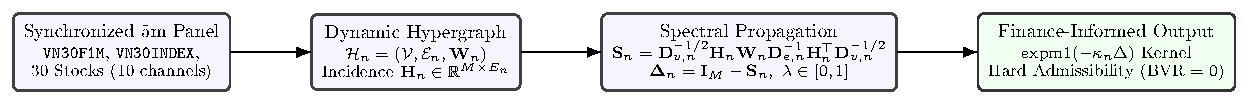
\includegraphics[width=0.98\linewidth]{fig_rc_fihgnn_pipeline.pdf}
  \caption{Phase 0 RC-FIHGNN data-to-admissibility pipeline mapping synchronized 5-minute futures, index, and 30-stock order-flow channels through dynamic hypergraph incidence, normalized spectral propagation, and hard economic admissibility projection.}
  \label{fig:pipeline}
\end{figure}

\section{Empirical Audit and Numerical Verification}
\label{sec:experiments}

\subsection{Gate G0 Synchronized 5-Minute Market Audit}
\label{sec:exp_audit}

\Cref{tab:g0_audit} reports the Phase~0 Gate~G0 data-routing audit across the synchronized 5-minute \texttt{ohlcv-dev} feed. Both \texttt{VN30F1M} (74,256 bars over 1,516 trading days) and \texttt{VN30INDEX} (50,761 bars over 1,059 trading days), together with all 30 active constituent equities (50 stocks in historical union), achieve $100\%$ completeness across all 10 price, volume, buy-up/sell-down order-flow, and foreign-flow channels.

\begin{table}[t]
  \centering
  \caption{Gate G0 synchronized 5-minute market panel audit across 10 OHLCV, order-flow, and foreign-flow channels.}
  \label{tab:g0_audit}
  \begin{tabular}{lcccc}
    \toprule
    Market Series & 5m Bars & Trading Days & Avg Bars/Day & Coverage (\%) \\
    \midrule
    \texttt{VN30F1M} Futures & 74,256 & 1,516 & 48.98 & 100.0 \\
    \texttt{VN30INDEX} Spot & 50,761 & 1,059 & 47.93 & 100.0 \\
    Active Basket (30 Stocks) & -- & -- & -- & 100.0 \\
    \bottomrule
  \end{tabular}
\end{table}

\subsection{Analytical and Monte Carlo Verification}
\label{sec:exp_math}

We verify every Phase~0 analytical claim numerically. First, exact cost-of-carry affine factorization yields $0.0$ residual under both continuous yields and discrete dividends, while the log-basis upper bound across 10,000 randomized trials exhibits a maximum remainder of $0.640735$ bps. Second, across 12 dyadic refinements ($m = 0, \dots, 11$), the discrete hedging discrepancy decays from $0.03556$ to $1.93 \times 10^{-5}$, attaining a final empirical convergence order of $0.999922$ against the theoretical order of $1.00$ (\Cref{fig:convergence}a).

\begin{figure}[t]
  \centering
  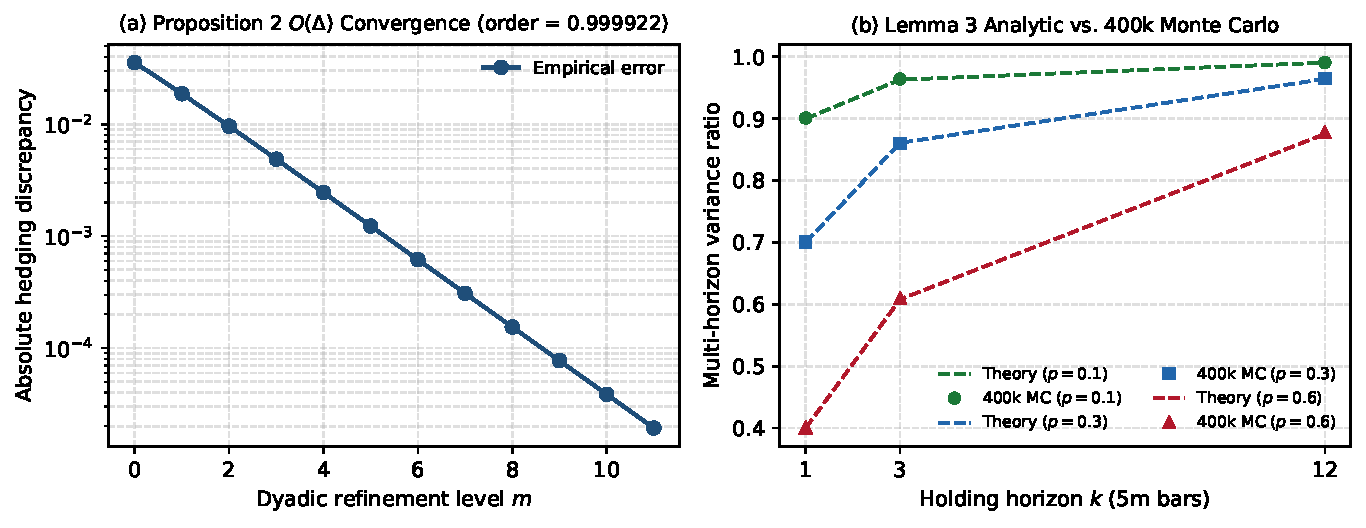
\includegraphics[width=0.98\linewidth]{fig_phase0_convergence.pdf}
  \caption{Empirical verification of Phase 0 analytical bounds: (a) 12-level dyadic refinement confirming first-order $O(\Delta)$ discrete hedging convergence with empirical slope $0.999922$, and (b) 400,000-path Monte Carlo agreement with closed-form multi-horizon variance ratios across $k \in \{1, 3, 12\}$.}
  \label{fig:convergence}
\end{figure}

\begin{table}[t]
  \centering
  \caption{Multi-horizon variance-ratio verification comparing closed-form Lemma 3 values against 400,000 Monte Carlo paths across decay parameter $p$ and holding horizon $k$.}
  \label{tab:lemma3_mc}
  \begin{tabular}{ccccc}
    \toprule
    Decay $p$ & Horizon $k$ & Monte Carlo Ratio & Analytic Ratio & Absolute Error \\
    \midrule
    0.1 & 1 & 0.90107 & 0.90000 & 0.00107 \\
    0.1 & 3 & 0.96420 & 0.96300 & 0.00120 \\
    0.1 & 12 & 0.99077 & 0.99074 & 0.00003 \\
    \midrule
    0.3 & 1 & 0.70086 & 0.70000 & 0.00086 \\
    0.3 & 3 & 0.86012 & 0.86100 & 0.00088 \\
    0.3 & 12 & 0.96464 & 0.96429 & 0.00036 \\
    \midrule
    0.6 & 1 & 0.40019 & 0.40000 & 0.00019 \\
    0.6 & 3 & 0.60927 & 0.60800 & 0.00127 \\
    0.6 & 12 & 0.87739 & 0.87527 & 0.00211 \\
    \bottomrule
  \end{tabular}
\end{table}

Third, \Cref{tab:lemma3_mc} and \Cref{fig:convergence}b confirm close agreement between closed-form multi-horizon variance ratios and 400,000 Monte Carlo trajectories across all 9 $(p, k)$ configurations. Fourth, at stiffness $x = 10^{-13}$, the $\operatorname{expm1}$ transition kernel achieves an absolute error of $1.11 \times 10^{-16}$ compared to $2.44 \times 10^{-4}$ under naive evaluation. Finally, across randomized hypergraph incidences and 10,000 fuzz trials, propagation symmetry holds to $2.78 \times 10^{-17}$, eigenvalues of $\boldsymbol{\Delta}_n$ remain inside $[0.0, 1.0]$, closed-form Gaussian CRPS matches quadrature within $6.51 \times 10^{-19}$, and hard admissibility achieves a $0.00\%$ bound-violation rate.

\section{Conclusion}
\label{sec:conclusion}

We presented and verified the Phase~0 mathematical and empirical data foundations for Regime-Conditioned Finance-Informed Hypergraph Learning in intraday index futures markets. Synchronized 5-minute data auditing across \texttt{VN30F1M}, \texttt{VN30INDEX}, and 30 constituent equities, paired with deterministic numerical verification of cost-of-carry parity, $O(\Delta)$ discrete hedging convergence, $\operatorname{expm1}$ numerical conditioning, and spectral admissibility of $\boldsymbol{\Delta}_n$, establishes a rigorous foundation for full multi-horizon empirical training and execution-aware hedging evaluation.


\bibliographystyle{plainnat}
\bibliography{references}

\end{document}
